%
\documentclass[conference]{IEEEtran}
\usepackage{url}
\usepackage{listings}
\usepackage{graphicx}
% \usepackage{hyperref}
\usepackage{caption}
\usepackage{subcaption}
\usepackage{multirow}
% *** GRAPHICS RELATED PACKAGES ***
%
\ifCLASSINFOpdf
  % \usepackage[pdftex]{graphicx}
  % declare the path(s) where your graphic files are
  % \graphicspath{{../pdf/}{../jpeg/}}
  % and their extensions so you won't have to specify these with
  % every instance of \includegraphics
  % \DeclareGraphicsExtensions{.pdf,.jpeg,.png}
\else
  % or other class option (dvipsone, dvipdf, if not using dvips). graphicx
  % will default to the driver specified in the system graphics.cfg if no
  % driver is specified.
  % \usepackage[dvips]{graphicx}
  % declare the path(s) where your graphic files are
  % \graphicspath{{../eps/}}
  % and their extensions so you won't have to specify these with
  % every instance of \includegraphics
  % \DeclareGraphicsExtensions{.eps}
\fi
% correct bad hyphenation here
\hyphenation{op-tical net-works semi-conduc-tor}
% 
\begin{document}
%
% paper title
% can use linebreaks \\ within to get better formatting as desired
\title{Demo Abstract \\ Use the Force, Luke \\
{\LARGE Implementation of RF-based gesture interaction on an android phone}}
% 
% author names and affiliations
% use a multiple column layout for up to three different
% affiliations
\author{
% \IEEEauthorblockN{Mathias Velten}
% \IEEEauthorblockA{Institute of Computer Science\\
% Georg-August-Universit\"at G\"ottingen\\
% matze@mathias-velten.de}
% \and
\IEEEauthorblockN{Christoph Rauterberg}
\IEEEauthorblockA{Institute of Computer Science\\
Georg-August-Universit\"at G\"ottingen\\
christoph@rauterberg.eu 
% Github: \url{https://github.com/crauterb/}
}
\and
\IEEEauthorblockN{Stephan Sigg, Xiaoming Fu}
\IEEEauthorblockA{Institute of Computer Science\\
Georg-August-Universit\"at G\"ottingen\\
\{sigg,fu\}@cs.uni-goettingen.de}}
% 
% make the title area
\maketitle
% 
\begin{abstract}
Various approaches exist to detect gestures and movements via smartphones. 
Most of them, however, require that the smartphone is carried on-body.
The abscence of reliable ad-hoc on-line gesture detection from environmental sources inspired this project for on-line hand gesture detection on a smartphone using only WiFi RSSI. 
We highlight our line of work and  explain problems at hand to provide information for possible future work.
We will furthermore introduce \emph{wifiJedi}, a smartphone application, that is able to detect movement in front of the smartphone by reading the WiFi RSSI and use this information to control a Slideshow.
\end{abstract}
% 
\IEEEpeerreviewmaketitle
% 

%  @TODO: Check all footnotes for correct numbering AFTER final formatting
% 
\section{Introduction}
% no \IEEEPARstartcognition
Over the last decade, smartphones have taken up an important role in our daily lives. 
With this growth in wealth of opportunities, the investigation of control mechanisms for smartphones has become an active research topic. 
The exploitation of the wide range of sensors that are included in mobile phones has spurred a multitude of interaction principles.
Gesture recognition over the wireless interface is, however, yet widely unexplored for mobile phones.
Gesture recognition from wireless signals was demonstrated with software defined radio (SDR) devices~\cite{Pervasive_Adib_2013,RFsensing_Pu_2013}.
Recently, it has also been shown how RSSI information from WiFi packets captured at a mobile phone can be exploited to detect gestures in proximity of the phone~\cite{RFSensing_Sigg_2014}.
While the former study exploited specialised hardware and the data in the latter work was processed offline, in this paper we present the first implementation of RSSI-based gesture recognition that runs completely on a mobile phone in real-time and with no external interface to the RF-channel. 
Furthermore we will describe lessons learned and give an outlook on possible future work, that could improve our results.

\section{Related Work}
When an object reflecting a signal wave is in motion, this causes Doppler Shift. 
The direction and speed of the movement conditions the strength and nature of this frequency shift.
Pu and others showed that simultaneous detection of gestures from multiple individuals is possible by utilising multi-antenna nodes and micro Doppler fluctuations~\cite{RFsensing_Pu_2013,RFsensing_Kim_2009}.
They utilise a USRP SDR multi antenna receiver and one or more single antenna transmitters distributed in the environment to distinguish between a set of 9 gestures with an average accuracy of 0.94. 
Their active device-free system exploits a MIMO receiver in order to recognise gestures from different persons present at the same time. 
By leveraging a preamble gesture pattern, the receiver estimates the MIMO channel that maximises the reflections of the desired user.

A main challenge was for them that the Doppler shift from human movement is several magnitudes smaller than the bandwidth of the signal employed.
The authors therefore proposed to transform the received signal into several narrowband pulses which are then analysed for possible Doppler fluctuation.
The group discussed application possibilities of their system in~\cite{RFSensing_Kellog_2014}.

In a related system, Adib and Katabi employ MIMO interference nulling and combine samples taken over time to achieve a similar result while compensating for the missing spatial diversity in a single-antenna receiver system~\cite{Pervasive_Adib_2013}.
In their system, they leverage standard WiFi hardware at 2.4GHz.

Later, this work was extended to 3D motion tracking by utlising three or more directional receive antennas in exactly defined relative orientation~\cite{RFSensing_Adib_2014}. 
In particular, the system is able to track the center of a human body with an error below 21cm in any direction and can also detect movement of body parts and directions of a pointing body part, such as a hand. 
This localisation is possible through time-of-flight estimation and triangulisation.
Higher accuracy of this estimation is granted by utilising frequency modulated carrier waves (sending a signal that changes linearly in frequency with time) over a bandwidth of 1.69GHz.
Impact of static objects could be mitigated by subtracting successive sample means whereas noise was filtered by its speed of changes in energy over frequency bands. 

Very recently, Sigg et al. investigated the distinction of gestures and situations in a passive device-free system with only one SDR~\cite{Pervasive_Sigg_2014b} or off-the-shelf smartphone~\cite{Pervasive_Sigg_2014,RFSensing_Sigg_2014} receiver.
They observed that 10 RSSI packets per second are sufficient to distinguish between simple classes and also hand gestures in proximity of the receiver.
Although the accuracy reached with purely WiFi-RSSI-based features was lower than for the USRP-systems exploiting Doppler fluctuation, they could distinguish 11 gestures performed in close proximity of the phone.

\section{Implementation}
In order to achieve a reliable on-line detection of movement and nearby gestures trough RSSI signal strengh information and to demonstrate its usage, we developed a show-case application for Android mobile phones.
The \emph{apk}\footnote{\url{user.informatik.uni-goettingen.de/~c.rauterberg}} and Source code\footnote{\label{footnoteImplementation}\url{https://github.com/crauterb/}} for the proposed application is available online. 
% The work flow of the application is illustrated in Figure~\ref{PCAN:flow}.
After setting up \emph{tcpdump}, data is collected, and parsed into a training set for the Machine learning algorithms before the trained classifier is used to control the slideshow.

%
\subsection{Platform Requirements}
The setup for the proposed \emph{wifiJedi} application requires a \emph{rooted smartphone} for access to system resources.
For this purpose, we used \emph{Cyanogenmod~7}\footnote{\url{http://wiki.cyanogenmod.org/w/Install_CM_for_passion}} on a \emph{Nexus One} phone.
Furthermore, we utilized the \emph{BCMon}\footnote{\url{http://bcmon.blogspot.de/2012/09/working-monitor-mode-on-nexus-one.html}} firmware in order to be able to access the WiFi interface of the phone in \emph{monitor mode}.
For this, it is mandatory that the hardware of the phone employs one of two widely instrumented broadcom chipsets (bcm4329 and bcm4330).
We also employed the library \emph{libsuperuser}\footnote{\url{http://su.chainfire.eu/}} in order to become able to issue terminal-commands as root from within an application.
%
\subsection{Data processing}
\subsubsection{Recording data}
%
The first choice for collecting RSSI information on Android Phones would be a \emph{Java}-library.
Yet, to our knowledge, all available libraries, do not suffice our needs: They do not capture all required data (e.g. sender, receiver, time, packet type) and, most significantly, provide average information rather than individual packet RSSI with an update frequency of not less than 1~Hz.
Therefore, we used the \emph{BCMon}-software to set the WiFi chip into \emph{monitoring mode} and then \emph{tcpdump} to capture data.
%
% As we wanted to run an online analysis on our \emph{Android}-phones, we were limited in our choice of programming languages.
% We used the \emph{bash}-program \emph{tcpdump} and called this program within the application.
% We recorded only information about the RSSI and SSID on the phone.
% Only interested in the RSSI-values and the SSID, we used the following \emph{tcpdump}-call:
% \begin{lstlisting}[language=bash,frame=single]
% tcpdump -vvv -e -ni eth0 -q -s0 -t
% \end{lstlisting}
% to collect our data. \\
%
% Can not s
We then parse all relevant information on the recorded packets from the output: % Can not say pcap files here, beacuse we parse from text file
\emph{RSSI}-values, source \emph{MAC}-address, packet type and the time stamp of the captured packets.
We utilised libsuperuser\footnotemark[5] in combination with the \emph{AsyncTask} class from the Android Developer Tools to run commands with root privileges without blocking the UI.
%
\subsubsection{Data analysis}
% The recorded data is exemplarily depicted in Figure~\ref{PCAN:touched}.
%
In order to improve recognition rates compared to previous work in the literature, we employ further features from the data.
\begin{enumerate}
\item The user will be asked to perform movements for a period of time $t$. 
This data will be recorded and stored into a file.
\item The recorded data will be divided into $n$ slots. 
Each packet is sorted into a slot according to its \emph{time stamp}.
\item We then use statistical analysis to compute the \emph{features} for Machine Learning. 
Those features are for one timeslot the \emph{statistical mean}, \emph{standard derivation}, \emph{highest} recorded RSSI value and \emph{lowest} recorded RSSI value, \emph{total number} of packets as well as \emph{numerical representation} of the source MAC-Addresses.

\item With these features, we use a \emph{k-nearest-neighbour}-Classifier to classify the data.
\end{enumerate}
All mentioned parameters can be set using the \emph{Settings}-Menu of the application. We will later describe the setup we used to achieve the presented results.
%
% \clearpage
%
\subsection{wifiJedi application}
We propose the \emph{wifiJedi} application that is able to detect movement in front of a smartphone using the WiFi RSSI.
It is a simple picture slideshow to demonstrate the RSSI-based gesture recognition.
The UI of the application is displayed in Fig.~\ref{pcan:UI}.
\begin{figure}
\centering
\begin{subfigure}[b]{0.2\textwidth}
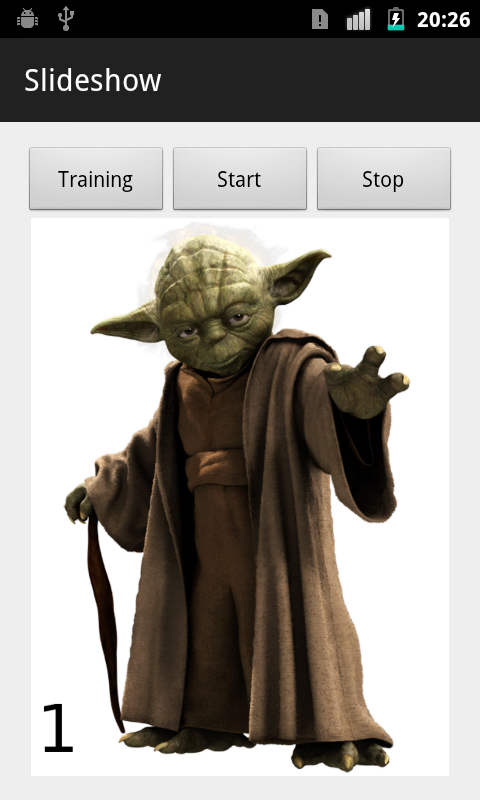
\includegraphics[width=\textwidth]{./pics/screen03}
\label{fig:screen_han}
\end{subfigure}%
~ %add desired spacing between images, e. g. ~, \quad, \qquad, \hfill etc.
%(or a blank line to force the subfigure onto a new line)
\begin{subfigure}[b]{0.2\textwidth}
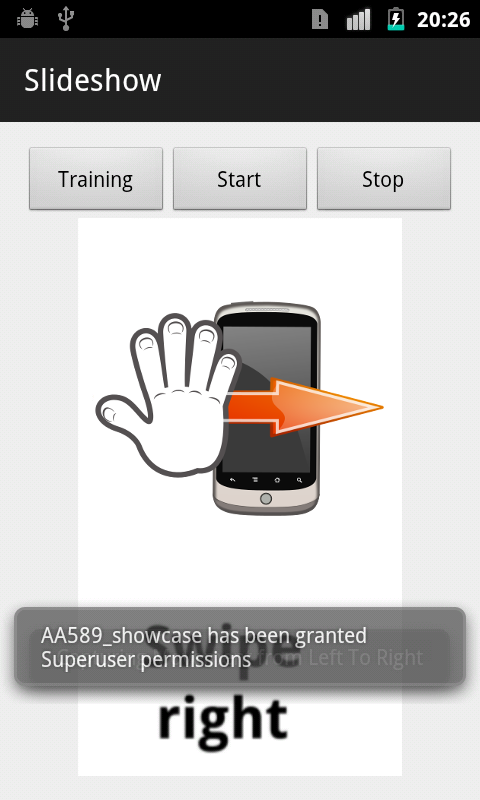
\includegraphics[width=\textwidth]{./pics/training}
\label{fig:screen_yoda}
\end{subfigure}
\caption{UI of the application (slideshow and training phase)}
\label{pcan:UI}
\end{figure}
%@TODO: Take correct pictures of the current UI!
Before it is started, the user will be asked to \emph{train} the application:
To distinguish between several classes, we need an example of those first. After the training is complete, the user can start the slideshow.
The different classes, that each represent a gesture, are displayed in Fig.~\ref{fig:classes}. 
\begin{figure}
\centering
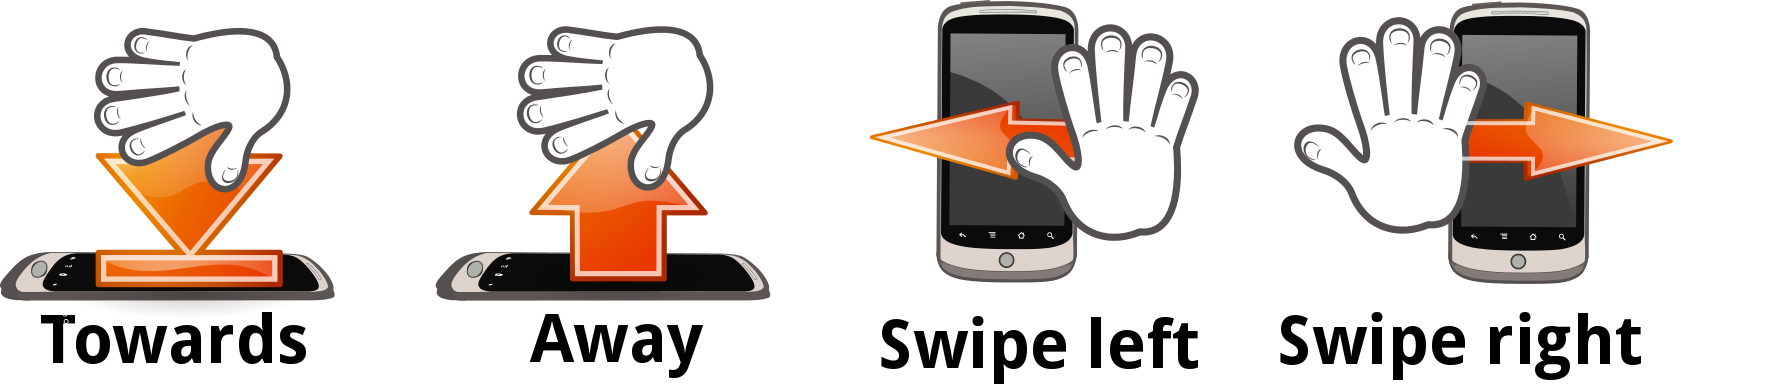
\includegraphics[width=.8\columnwidth]{./pics/gestures3}
\caption{All gestures considered. The Showcase Slideshow uses swipes over the phone to navigate within the slideshow. The corresponding classes are listed in Fig.~\ref{res:matrix}}
\label{fig:classes}
\end{figure}
Within the ``settings'' menu, the user can optimize several settings, that have proven to be relevant to the performance.
With a hand movement \emph{from left to right} or \emph{from right to left} the user then navigates trough the showcase slideshow.

\subsection{Demonstration setup}
The application is available online\footnote{\url{user.informatik.uni-goettingen.de/~c.rauterberg}} and will be part of any given presentation.
Users will be able to interact with a show case application by controlling the application via gestures.
For all purposes, we consider the \emph{GNU Free Documentation License} as on open source license.

\section{Evaluation of the proposed approach}
First, we will evaluate the default usage of the showcase slideshow: 
After a training phase, while holding the phone in the hand, we record test samples to evaluate the accuracy of the classification. 
We will refer to this scenario as the \emph{standard scenario}.
In addition, with two phones we tested the classification in different scenarios:
\begin{description}
\item[Training: ] We train the classifier whilst holding the phone \emph{on a certain spot in a certain room} and then \emph{walk about the room} and evaluate the classifier on different positions in the room.
\item[Ad-hoc:  ] We train the classifier whilst holding the phone \emph{on a certain spot in a certain room} and then \emph{completely leave the context} and go to other spaces within the city and evaluate the performance there. 
\end{description}
\subsection{Choice of parameters}
In all scenarios, we recorded $t=10\sec$ of training data for each of the classes. We divided this data into $n=40$ slots, resulting in $t_i=0.25\sec$ duration for each time slot. To avoid the affects of fluctuations in the networks traffic, we did not record $t=10\sec$ of packets for each class at once, but iteratively recorded only $2\sec$ for each class. For Machine Learning, we used \emph{k-nearest-neighbour} with $k=5$ neighbours. \\
The \emph{standard scenario} and the \emph{training scenario} were each tested with $125$ test runs, the \emph{ad-hoc scenario} was tested with $60$ test runs.
%
\section{Results}
\subsection{Results within the Showcase Slideshow}
Table~\ref{res:matrix} shows the confusion matrix of a validation in the \emph{Standard Scenario}. 
\begin{table}
\caption{The confusion matrix of a standard training phase. The movements corresponding to the classes are listed with the actual classes.}
\centering 
\renewcommand{\arraystretch}{1.5}
\begin{tabular}{cc|c|c|c|c|l}
\cline{3-6}
& & \multicolumn{4}{ c| }{Predicted Class} \\ \cline{3-7}
& & $C_1$ & $C_2$ & $C_3$ & $C_4$ &\multicolumn{1}{ |c| }{Recall} \\ \cline{1-7}
\multicolumn{1}{ |c  }{\multirow{4}{*}{\rotatebox{90}{Actual Class}} } &
\multicolumn{1}{ |c| }{$C_1 = Away$} & $0.88$ & $0.02$ & $0.04$ & $0.06$ &   \multicolumn{1}{ |c| }{$0.88$}  \\ \cline{2-7}
\multicolumn{1}{ |c  }{}                        &
\multicolumn{1}{ |c| }{$C_2 = Towards$} & $0.01$ & $0.91$ & $0.04$ & $0.04$ &  \multicolumn{1}{ |c| }{$0.91$}   \\ \cline{2-7}
\multicolumn{1}{ |c  }{} &
\multicolumn{1}{ |c| }{$C_3 = Swipe_{right}$} & $0.00$ & $0.02$ & $0.95$ & $0.03$ & \multicolumn{1}{ |c| }{$0.95$} \\ \cline{2-7}
\multicolumn{1}{ |c  }{}                        &
\multicolumn{1}{ |c| }{$C_4 = Swipe_{left}$} & $0.00$ & $0.01$ & $0.05$ & $0.94$ & \multicolumn{1}{ |c| }{$0.94$} \\ \cline{1-7}
 \multicolumn{1}{ c  }{}                        &
\multicolumn{1}{ |c| }{Prec.} & $0,98$ & $0,94$ & $0,87$ & $0,87$ &     \\ \cline{2-6}
\end{tabular}

\label{res:matrix}
\end{table}
We observe that the classes $C_3$ and $C_4$ are correctly identified with about $95 \%$ and that there is only a small number of \emph{false-positives} to these classes. 
The classes $C_1$ and $C_2$ are correctly identified with about $90 \%$. 
In Fig.~\ref{res:mean} we can see the \emph{statistical mean} over all relative \emph{true-positives} for all three scenarios. 
Here we observe that on average more than $90\%$ of the classes $C_3$ and $C_4$ are predicted correctly. \\
This means, that in both scenarios we are able to control the proposed showcase slide show via gestures.

\subsection{Results for the alternative scenarios}
Fig.~\ref{res:mean} shows, that in the \emph{Ad-hoc Scenario} the average amount of correct classifications suffers greatly, especially for the classes $C_1$ and $C_2$. This is due to the fact, that this approach is still \emph{very dependent on the current fluctuation within the network}:
The change in context, i.e. number of access points and fluctuation leads to a low accuracy of the learned classifier.


% This one version
\begin{figure}[tb]
\centering
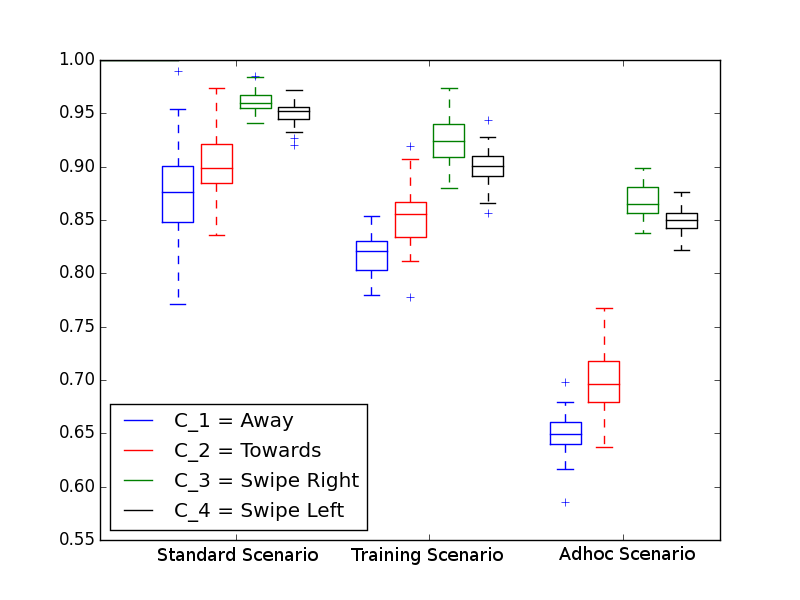
\includegraphics[width=0.85\columnwidth]{./pics/boxcompare}
% where an .eps filename suffix will be assumed under latex,
% and a .pdf suffix will be assumed for pdflatex; or what has been declared
% via \DeclareGraphicsExtensions.
\caption{An illustration off the averages of all experiments we did in all three described scenarios.}
\label{res:mean}
\end{figure}
%
% 
% 
\section{Summary \& Outlook on Future Work}
We have proposed a showcase application for online RF-based gesture interaction on Android devices. After initial training we are able to correctly classify certain gestures with an accuracy of about $95\%$.
In future work, we want to circumvent the long initial training by providing several \emph{scenarios} to the application. Upon starting, the application will \emph{analyze} the current network and provide a likelihood of the provided scenarios. 
% Furthermore, we will test the \emph{power consumption} in the proposed approach and compare it to other valid gesture recognition methods on smartphones.
%
\bibliographystyle{plain}
\bibliography{pcan}
%
% that's all folks
\end{document}


